% Plots



% Plot for constant noise
\def \constantNoisePlot 
{
\begin{axis}[%
	xmin=0,
	xmax=8000,
    xlabel={Agents evaluated},
    ylabel={stepsize},
    ymode=log,
    log basis y={10},
    width=16cm,
    height=12cm,
    legend pos=south east,
    title={},
    xticklabel = {
    \pgfmathparse{\tick/1000}
    \pgfmathprintnumber{\pgfmathresult}\,k
}]
\foreach \x in {0,1,2,3,4,5,6,7,8,9}
{
\addplot[color=black,mark=none]  
 table [x=agents, y=meanScore, col sep=comma]    
       {data/ConstantNoise/ce_ConstantNoise_\x.txt};
}
\end{axis}
}




% Plot for linear decreasing noise
\def \linearNoisePlot 
{
\begin{axis}[%
	xmin=0,
	xmax=8000,
    xlabel={Agents evaluated},
    ylabel={stepsize},
    ymode=log,
    log basis y={10},
    width=16cm,
    height=12cm,
    legend pos=south east,
    title={},
    xticklabel = {
    \pgfmathparse{\tick/1000}
    \pgfmathprintnumber{\pgfmathresult}\,k
}]
\foreach \x in {0,1,2,3,4,5,6,7,8,9}
{
\addplot[color=black,mark=none]  
 table [x=agents, y=meanScore, col sep=comma]    
       {data/LinearNoise/ce_LinearNoise_\x.txt};
}
\end{axis}
}



% Plot for constant noise
\def \noNoisePlot
{
\begin{axis}[%
	xmin=0,
	xmax=8000,
    xlabel={Agents evaluated},
    ylabel={stepsize},
    ymode=log,
    log basis y={10},
    width=16cm,
    height=12cm,
    legend pos=south east,
    title={},
    xticklabel = {
    \pgfmathparse{\tick/1000}
    \pgfmathprintnumber{\pgfmathresult}\,k
}]
\foreach \x in {0,1,2,3,4,5,6,7,8,9}
{
\addplot[color=black,mark=none]  
 table [x=agents, y=meanScore, col sep=comma]    
       {data/NoNoise/ce_NoNoise_\x.txt};
}
\end{axis}
}


% Plot for means
\def \meansPlot 
{
\begin{axis}[%
	xmin=0,
	xmax=8100,
    xlabel={Iteration/Generation},
    ylabel={Mean score},
    ymode=log,
    log basis y={10},
    width=\textwidth,
    height=12cm,
    legend pos=south east,
    xticklabel = {
    \pgfmathparse{\tick/1000}
    \pgfmathprintnumber{\pgfmathresult}\,k
}]
\addplot[color=black,mark=none, dotted, thick] 
    table [x=agents, y=meanScore, 
           col sep=comma] {data/NoNoise/mean.txt};
\addplot[color=black,mark=none, thick] 
    table [x=agents, y=meanScore, 
           col sep=comma] {data/ConstantNoise/mean.txt};
\addplot[color=black,mark=none,dashed, thick] 
    table [x=agents, y=meanScore, 
           col sep=comma] {data/LinearNoise/mean.txt};
\legend{No noise, constant noise, Linear decreasing noise}
\end{axis}
}

% Plot for first comparison between CMA-ES and CE-Constant noise
\def \cmaCePlot
{
\begin{axis}[%
	xmin=0,
	xmax=8000,
    xlabel={Number of agents evaluated},
    ylabel={Mean score},
    ymode=log,
    log basis y={10},
    width=\textwidth,
    height=12cm,
    legend pos=south east,
    xticklabel = {
    \pgfmathparse{\tick/1000}
    \pgfmathprintnumber{\pgfmathresult}\,k
}]
\addplot[color=black,mark=none, dashed, thick] 
    table [x=agents, y=meanScore, 
           col sep=comma] {data/ConstantNoise/mean.txt};
\addplot[color=black,mark=none,thick] 
    table [x=agents, y=score, 
           col sep=comma] {data/CMA_00/cma_sigma_0_5_mean.txt};
\legend{Cross Entropy ($z_t = 4$ $\sigma_0 = 100$), CMA-ES ($\sigma_0 = 0.5$)}
\end{axis}
}


\def \plotBertsekasCmaVsCEHardTetris
{
\begin{axis}[%
	xmin=0,
	xmax=8000,
    xlabel={Agents evaluated},
    ylabel={Mean Score},
    ymode=log,
    log basis y={10},
    width=16cm,
    height=12cm,
    legend pos=south east,
    title={Bertsekas comparison, hard Tetris},
    xticklabel = {
    \pgfmathparse{\tick/1000}
    \pgfmathprintnumber{\pgfmathresult}\,k
}]
\addplot[color=black,mark=none,dashed, very thin]  
 table [x=agents, y=meanScore, col sep=comma, ] 
 {data/FeaturesetCompare/_ce_bert_hard_ConstantNoise_mean.txt};
\addplot[color=black,mark=none, very thin]  
 table [x=agents, y=meanScore, col sep=comma, ] 
 {data/FeaturesetCompare/_cma_bert_hard_mean.txt};
\legend{Cross Entropy ($z_t = 4$ $\sigma_0 = 100$), CMA-ES ($\sigma_0 = 1$)}
\end{axis}
}

\def \plotDellCmaVsCEHardTetris
{
\begin{axis}[%
	xmin=0,
	xmax=8000,
    xlabel={Agents evaluated},
    ylabel={Mean Score},
    ymode=log,
    log basis y={10},
    width=16cm,
    height=12cm,
    legend pos=south east,
    title={Dellacherie comparison, hard Tetris},
    xticklabel = {
    \pgfmathparse{\tick/1000}
    \pgfmathprintnumber{\pgfmathresult}\,k
}]
\addplot[color=black,mark=none,dashed, very thin]  
 table [x=agents, y=meanScore, col sep=comma, ] 
 {data/FeaturesetCompare/_ce_dell_ConstantNoise_mean.txt};
\addplot[color=black,mark=none, very thin]  
 table [x=agents, y=meanScore, col sep=comma, ] 
 {data/FeaturesetCompare/_cma_dell_hard_mean.txt};
\legend{Cross Entropy ($z_t = 4$ $\sigma_0 = 100$), CMA-ES ($\sigma_0 = 1$)}
\end{axis}
}



\newcommand{\plotCEConfig}[3]
{
\begin{tikzpicture}
\begin{axis}[%
	xmin=0,
	xmax=8000,
	ymin=0,
	ymax=1000000,
    xlabel={},
    ylabel={},
    ymode=log,
    log basis y={10},
    width=8cm,
    height=6cm,
    legend pos=south east,
    title={$\populationSize = #1, \offspringNumber=#2$},
    xticklabel = {
    \pgfmathparse{\tick/1000}
    \pgfmathprintnumber{\pgfmathresult}\,k
}]
\foreach \x in {0,1,2,3,4,5,6,7,8,9}
{
\addplot[color=black,mark=none, very thin]  
 table [x=agents, y=meanScore, col sep=comma, ] {data/CrossEntropyConfiguration/#3\x.txt};
}
\end{axis}
\end{tikzpicture}
}

\newcommand{\plotCEConfigBase}[3]
{
\begin{tikzpicture}
\begin{axis}[%
	xmin=0,
	xmax=8000,
	ymin=0,
	ymax=1000000,
    xlabel={},
    ylabel={},
    ymode=log,
    log basis y={10},
    width=8cm,
    height=6cm,
    legend pos=south east,
    title={$\populationSize = #1, \offspringNumber=#2$},
    xticklabel = {
    \pgfmathparse{\tick/1000}
    \pgfmathprintnumber{\pgfmathresult}\,k
}]
\foreach \x in {0,1,2,3,4,5,6,7,8,9}
{
\addplot[color=black,mark=none, very thin]  
 table [x=agents, y=meanScore, col sep=comma, ] {#3\x.txt};
}
\end{axis}
\end{tikzpicture}
}



\def \ellipseFigure{
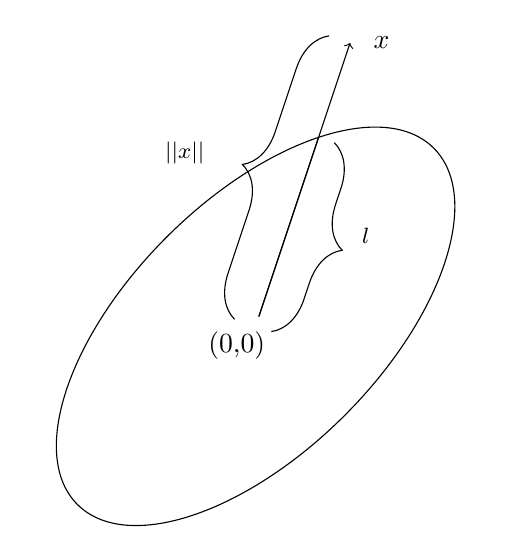
\begin{tikzpicture}[scale=0.8]
\draw  [rotate=45] (0,0) node (v1) {} ellipse (4 and 2);
\draw (v1) -- (1,3);
\draw [->] (v1) -- (1.5,4.5);
\draw [decorate,decoration={brace,amplitude=15pt,mirror,raise=6pt},yshift=0pt]
(0,0) -- (1,3) node [black,midway,xshift=1cm,yshift=-1.4] {\footnotesize
$l$};
\draw [decorate,decoration={brace,amplitude=15pt,raise=8pt},yshift=0pt]
(0,0) -- (1.5,4.5) node [black,midway,xshift=-1.5cm,yshift=0.4cm] {\footnotesize
$||x||$};
\node at (2,4.5) {$x$};
\node at (-0.3,-0.3) {(0,0)};
\end{tikzpicture}
}



